\documentclass[a4paper,twocolumn]{article}

\usepackage[left=1in, right=1in, top=0.5in, bottom=1in]{geometry}

\usepackage{siunitx}
\usepackage{hyperref}
\usepackage{circuitikz}
\usepackage{amsmath}
\usepackage{amsfonts}
\usepackage{mathtools}
\usepackage{physics}

\usepackage{import}
\usepackage{xifthen}
\usepackage{pdfpages}
\usepackage{transparent}
\usepackage{titlesec}


\newcommand{\incfig}[1]{
    \def\svgwidth{\columnwidth}
    \import{./figures/}{#1.pdf_tex}
}

\titlespacing*{\abstract}
{0pt}{0pt}{10pt}

{\renewenvironment{abstract}{%
       \if@twocolumn
         \section*{\abstractname}%
       \else
         \small
         \paragraph{\abstractname:}
       \fi}
       {\if@twocolumn\else\par\bigskip\fi}}


\title{FP09 - Neuromorphic computing}
\author{\textbf{Students: }R. Dorstijn (sd249) \& Moritz Epping (hh234) \\ \textbf{Tutor: }Jakob Kaiser}
\date{February 2021}

\begin{document}
\maketitle

\twocolumn[
  \begin{@twocolumnfalse}
    \begin{abstract}
        This paper presents a review of the SPIKEY chip for neuromorphic
        computing.  After a theoretical framework outlining the requirements
        for a simple neuromorphic computing device has been given, this
        specific hardware realization will be examined under these considerations.
        It will be shown that the SPIKEY chip exhibits all of the basic functions
        of neuromorphic hardware and is reliable for simple experiments.  Employing
        this chip for actual applications such as computations however is not
        advisable since production errors significantly alter the chip's behaviour
        in a non-trivial way and environmental factors such as temperature
        fluctuations have an equally important effect on making the chip
        unreliable for large-scale applications.  A procedure to counter
        some of these effects will be provided.
    \end{abstract}
  \end{@twocolumnfalse}
]
\section{Motivation and Theory}
\subsection{Motivation}
Brains and computers often are compared because of their shared purpose:
decision making, though they have irreconcilable differences in architecture.
Modern computers function on the basis of the van Neumann
architecture\cite{von-Neumann}, which separates the control unit from the memory
and the computation unit. Though this simplifies the structure of the computer and
makes it modular, it does however create a clear bottleneck at the communication layer,
commonly known as the von Neumann bottleneck. This creates an energy
inefficiency that is unacceptable for biological systems like that of
humans, who spend around 20\% of their total energy uptake on the brain\cite{metabolic-rates}.
This most likely has provided significant evolutionary pressure for hominids to
optimize metabolic resource usage\cite{seymour2016fossil}.  For this reason a new
architecture for computers has been suggested: neuromorphic\footnote{``Neuro''
as in brain, ``-morphic'' as in having the shape of, forming ``having the shape
of a brain''.} computing.  Besides more efficient energy usage,  the scientific
interest in neuromorphic computing is also grounded in the idea of trying to
understand the human brain by rebuilding it artificially.

\subsection{Signal processing in the brain}
Neurons are the basic computational components of the
brain, transmitting and morphing signals. Each neuron receives signals from
others at the dendrites, which shift the electric potential at the membrane of
the cell at the site of the synapse\footnote{The connection point of two
dendrites where the axon of one meets the dendrite of the other.}, creating an
ion wave crossing the entire membrane of the neuron, reaching it's axon,
allowing it to pass the signal on to other neurons.

The potential at the neuron membrane as a function of time has three main
domains: there is the rest voltage, where the potential is constant, there is
the peak, which looks roughly Gaussian and then there is a short period that the
membrane is hyperpolarized, meaning that it is so negatively charged that new
signals do not instigate a new response.

% \begin{figure}[ht]
%     \centering
%     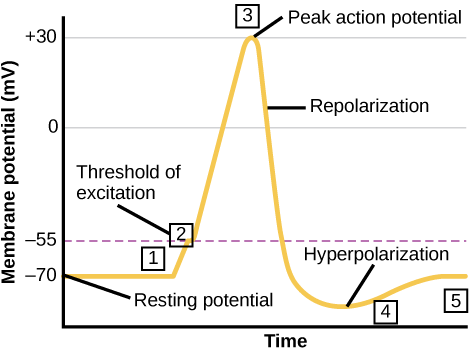
\includegraphics[width=.5\textwidth]{figures/action-potential.png}
%     \caption{Formation of an action potential. Source:  \url{https://courses.lumenlearning.com/boundless-biology/chapter/how-neurons-communicate/}}
%     \label{fig:action-potential}
% \end{figure}

\subsection{The LIF model}
In order to emulate the behaviour electronically, a leaky integrate and fire
(LIF) model is used. A single neuron is represented by an electronic circuit
like the one in figure \ref{fig:circuit}. When the chip is not excited, nor
inhibited there is a constant ``leak'' voltage present on the membrane,
representing the biological rest potential of the membrane potential.  The neuron,
represented as a capacitor with capacitance $C_m$ is charged and decharged
by the input of other neurons. With constant excitatory (facilitating spikes) and
inhibitory (suppressing spikes) potential,  all dynamics are encoded in the
time-dependent conductances $g_j(t),  g_x(t)$.  A spike coming from either
of these two synapses is implemented by temporarily increasing the corresponding
conductance.  When the threshold voltage $V_\text{thres}$,  is reached,
the amplifier functioning as a comparator in this setting,  sends out a
$V_{CC}$ signal to a digital unit that processes that the neuron has fired
and is responsible for closing the switch that keeps the
``membrane potential'' $V_m$ at some $V_\text{reset}$ for the refractory
period. This time is meant to mimic the period the voltage at the membrane
increases non-linearly and therefore loses its sensitivity to input. The digital
processing unit is also responsible for sending the signal (in terms of a
uniform spike; ''All-or-nothing reponse'') to the neurons that the are
connected to one that just fired.  The synapses then transform this voltage
spike into an excitatory or inhibitory input for the other neurons.

\begin{figure}[ht]
    \centering
    \begin{circuitikz}[scale = .6, transform shape]
        \draw (0, 0)    to node[midway, above]{$V_m$} (8.5, 0) node[op amp, anchor=+](A1){}; % main line
        \draw (A1.out)  to[short, l=$V_\text{out}$, -o] ++(1, 0);
        \draw (7, 1)    node[left, above] {$V_\text{thres}$} to[short, *-] (A1.-);
        \draw (0, 0)    to[vR, l=$g_l$, *-] (0, -2)
                        to[battery1, l=$E_l$] (0, -3) node[ground] {} (0, -4);
        \draw (2, 0)    to[vR, l=$g_x$, *-] (2, -2)
                        to[battery1, l=$E_x$] (2, -3) node[ground] {} (2, -4);
        \draw (4, 0)    to[vR, l=$g_i$, *-] (4, -2)
                        to[battery1, l=$E_g$] (4, -3) node[ground] {} (4, -4);
        \draw (6, 0)    to[C, l=$C_m$] (6, -2)
                        node[ground] {} (6, -2);
        \draw (8, -3)   to[short, l_=$V_\text{reset}$, o-] (8, -1)
                        to[normal open switch, -*] (8, 0);
        \draw (7.5, -2) node[anchor=north] {$V_\text{reset}$}
                        to[short, o-] (7.5, -1)
                        to[normal open switch, -*] (7.5, 0);
        \draw [densely dashed]
              (3.3, -4) --++(0, 4.6)
                        --++(5, 0)
                        --++(0, -4.6)
                        --++(-5, 0);
    \end{circuitikz}
    \caption{Circuit of a single neuron in a LIF chip.}
    \label{fig:circuit}
\end{figure}

\section{Execution \& Results}
Having laid out the theoretical foundations and characteristics each device
for neuromorphic computing should exhibit,  it now needs to be investigated
whether the hardware at hand fulfills these requirements.  This process begins
by investigating the most simple behaviour and only once it has been validated
that this behaves as expected more complicated setups such as networks
can be analyzed.
A rather interesting setup was provided by the university of Heidelberg. It
hosted a SPIKEY chip on its grounds, which was physically inaccessible due to
the COVID-19 crisis, therefore it was connected to a job manager that could be
written to by the Jülich Supercomputing Center, which hosted Jupyter notebooks
for this purpose. A SPIKEY chip implements the LIF model physically.

\subsection{Investigation of a single neuron}
%% Moritz  %%
A single neuron will be investigated,  without considering any excitatory or
inhibitory inputs.  This reduces the circuit of figure \ref{fig:circuit}
to the dashed square drawn inside of it. The relevant parameters
that appear in figure are:
\begin{itemize}
    \item $E_l$ setting the \textit{amount} of potential leaking into the `membrane'.
    \item $g_l$ determining how \textit{quickly} the potential leaks into the `membrane'.
    \item $C_m$ describing how much potential is leaked to ground.
    \item $V_\text{reset}$ prescribing the starting point of a cycle.
\end{itemize}

Our final goal is to determine whether the spikey chip is a suitable hardware for
neuromorphic computing.  Before eventually testing the chip in configurations
that are actually capable of computations,  it is sensible to verify that the
most basic circuit is working as desired.  Hence we split the LIF model circuit
and only consider a neuron without output (neither excitatory nor inhibitory).
By setting the leakage potential above the threshold, we bring the circuit into
a continuous firing regime. \par
\textit{Threshold Voltage} $V_{th}$ and \textit{reset voltage} $E_r$ can be
specified by the user.  We run the circuit,  record the voltage of a neuron as
a function of time and plot our results.

\begin{figure}[ht]
    \centering
    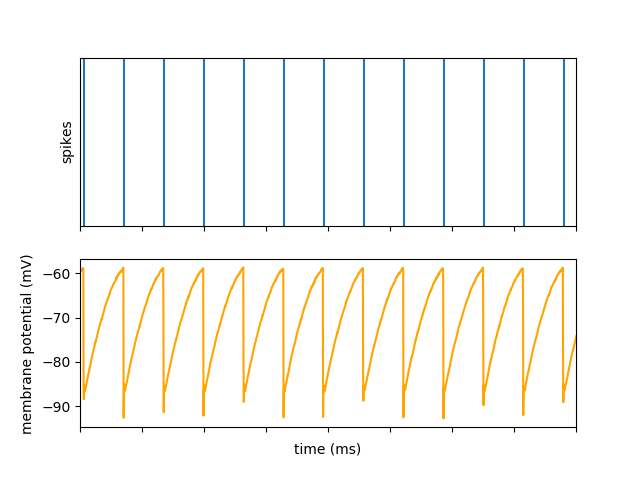
\includegraphics[width=.5\textwidth]{figures/fp_task1_1membrane.png}
    \caption{Voltage over a single neuron with leakage potential over threshold potential}
    \label{fig:membranes_ex1}
\end{figure}

The threshold voltage of $V_{th} = -55$ mV was approached up to $5$ mV.  The
reset voltage of $E_r = -80$ mV was not precisely reached.  After each recovery
of the voltage we observed strong fluctuations of the reset voltage.  We
furthermore calculated the time between spikes and found a value of
$t_{fir} = (16.10\pm 0.11)$ ms.  From figure \ref{fig:membranes_ex1} it becomes 
apparent that in this simple setup the neuron behaves as a capacitor that is
being charged.  The firing rate could be increased by increasing either the
leakage conductance,  leakage voltage or threshold voltage or by decreasing
the capacitance of the LiF circuit.

\subsection{Calibrating neuron parameters}
%% Robin  %%

%theory
In the case of a single unconnected neuron the membrane potential can be
understood with application of the Kirchoff formula to the circuit in the dashed
box of figure \ref{fig:circuit}.
\[
    C_m \frac{dV_m}{dt} = g_l(E_l - V_m)
\]
Clearly, this is a ordinary first order differential equation and has the
solution
\begin{equation}
    V_m(t) = A \exp(\frac{-g_l}{C_m}t) - E_l
    \label{eq:diff-eq-sol}
\end{equation}
where $A$ is given by the initial condition:
\[
    A = V_m(0) - E_l.
\]

In order to set a neuron to fire at a regular frequency $\tau_m$, we have to take
into account that $V_m$ will be reset to $V_\text{reset}$ when it hits
$V_\text{thres}$. Equation \eqref{eq:diff-eq-sol} can be rephrased in terms of
$t$.
\begin{equation}
    \tau_m = -\ln(\frac{V_\text{thres} - E_l}{V_\text{reset} - E_l})
    \frac{C_m}{g_l}
    \label{eq:tau}
\end{equation}

The characteristic time constant $\tau_c$ of the system can be found by setting
$V_\text{thres}$ as a function of $E_l$ and $V_\text{reset}$.
\[
    V_\text{thres} = E_l - (E_l - V_\text{reset})\exp(-1)
\]
The resulting $\tau_c$ is then only dependent on $C_m$ and $g_l$:
\begin{align*}
    \tau_m &= -\ln(\frac{E_l - (E_l - (E_l - V_\text{reset})\exp(-1))}{V_\text{reset} - E_l}) \frac{C_m}{g_l}\\
           &= -\ln(\frac{(E_l - V_\text{reset})\exp(-1))}{V_\text{reset} - E_l})\frac{C_m}{g_l} \\
           &= \frac{C_m}{g_l} = \tau_c
\end{align*}
This time constant does not take into account the refractory period which should
adds a fixed contribution. This was mentioned in equation \eqref{eq:tau}, but
becomes relevant again when considering the total time.

This describes a good theory of the neuron, however in reality there are some
serious production artifacts that require calibration.

% execution
On the SPIKEY chip 4 neurons were isolated programmatically and given the same
parameters:
\begin{itemize}
    \item $V_\text{reset}$: \SI{-80.0}{\milli\volt}
    \item $V_\text{thresh}$: \SI{-55.0}{\milli\volt}
    \item $E_\text{leak}$: \SI{-50.0}{\milli\volt}
    \item $g_\text{leak}$:  \SI{20.0}{\nano\siemens}
\end{itemize}

This however resulted in wildly differing frequencies. In order to compensate
for this $g_l$ was adjusted individually for all of the membranes so that they
were all correct within their respective standard deviation:
\SI{20.1}{\milli\volt}, \SI{55.0}{\milli\volt}, \SI{60.0}{\milli\volt},
\SI{20.5}{\milli\volt}.

The scale of the problem becomes even more clear when considering the that one
half of the SPIKEY chip has a rate distribution like presented in figure
\ref{fig:distribution}, the previous method of trial and error becomes rather
infeasible.

\begin{figure}[ht]
    \centering
    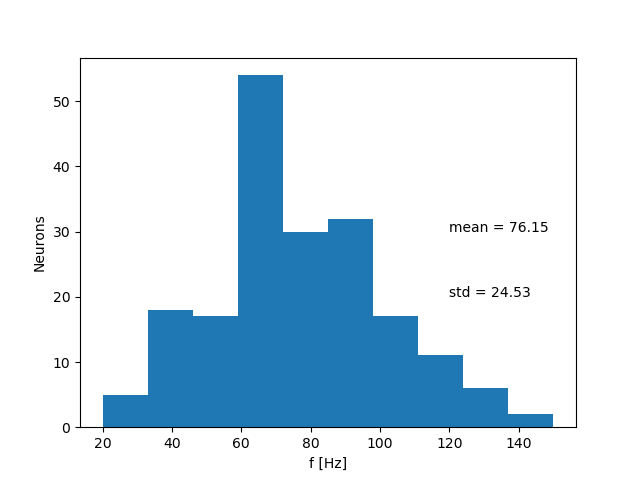
\includegraphics[width=.5\textwidth]{figures/rate-distribution.png}
    \caption{Distribution of firing rate for the same across one side of the
    chip.}
    \label{fig:distribution}
\end{figure}

Instead an algorithm is suggested that should help find a proper calibration for
all neurons that are able to converge on the desired rate.
\begin{enumerate}
    \item Set the $g_l$ to the default value and measure the rate of the neuron.
    \item Set the $g_l$ to double the default value and measure the rate of the
        neuron.
    \item Describe the response of the neuron linearly using the last two
        points and estimate where the desired rate would lie.
    \item Set the $g_l$ to this value and measure the rate, if it is within the
        standard error: success! If not return to step 3.
\end{enumerate}
Sadly we were unable to implement the algorithm, but we encourage the reader
to.

\subsection{A Single Neuron with Synaptic Input}
Interconnectivity between neurons is crucial since this forms the basis of
computations.  We now want to evaluate how a single neuron behaves under the influence
 of synaptic input.  To do that,  we stimulate one hardware neuron with a synapse
 and record its membrane potential.  The readout signal is subject to significant
 noise which is due to the read-out process.  Stimulating the neuron with a regular
 spike train allows us to average out these fluctuations.  The spike triggered average
 height of the post synaptic potentials is a good measure of the strength of the signal.
 Furthermore,  we measure the time scale on which the potential decays.
The parameters determining the shape of the synaptic conductance can be chosen
from these ranges:
\begin{align*}
	\text{drviout} &\in \left[ 0.013, 1.667  \right] \\
	\text{drvifall} &\in \left[ 0.02,  2.5  \right]
\end{align*}
We pick as default values approximately the mean of these intervals and
investigate for each parameter both extremes.  Default: $\text{drviout} := 0.80$
and $\text{drvifall}=1.3$.
% \begin{figure}[ht]
%     \centering
%     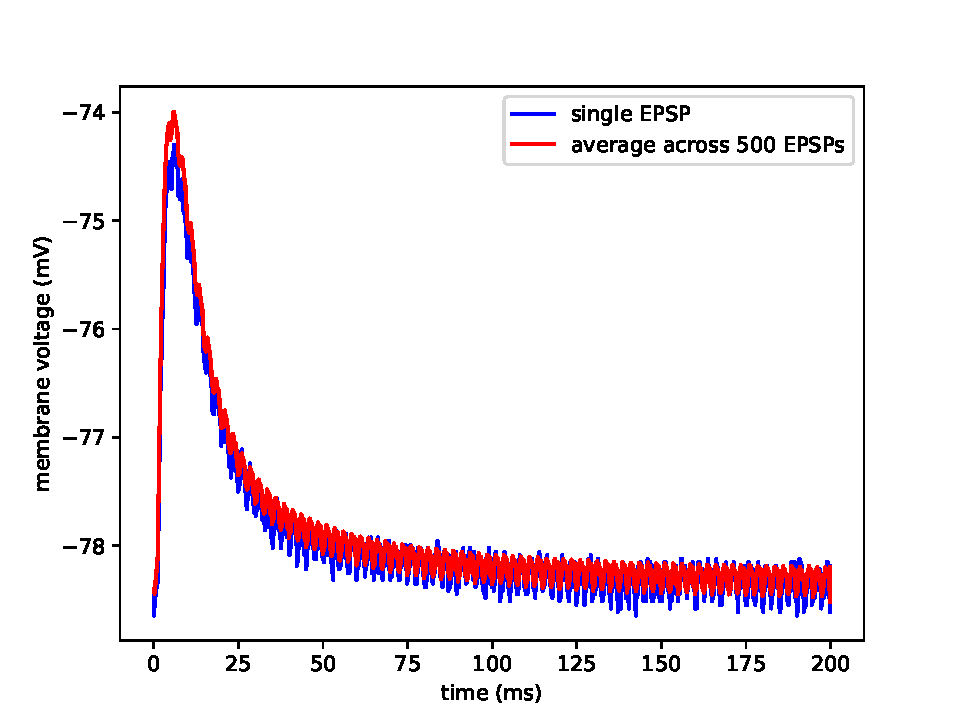
\includegraphics[width=.5\textwidth]{figures/epsp_default.pdf}
%     \caption{Post synaptic potential for default settings of parameters}
%     \label{fig:epsp_default}
% \end{figure}
%\begin{figure}[ht]
    %\centering
    %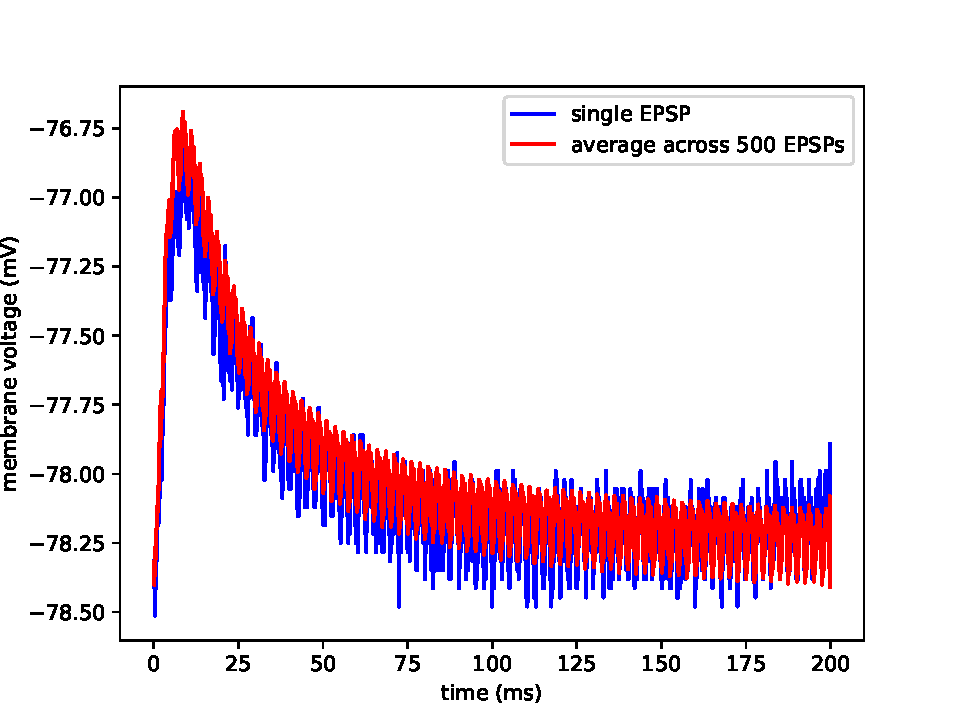
\includegraphics[width=.5\textwidth]{figures/epsp_out_-.pdf}
   % \caption{EPSP for low drviout.}
   % \label{fig:epsp_out-}
%\end{figure}
%\begin{figure}[ht]
 %   \centering
 %   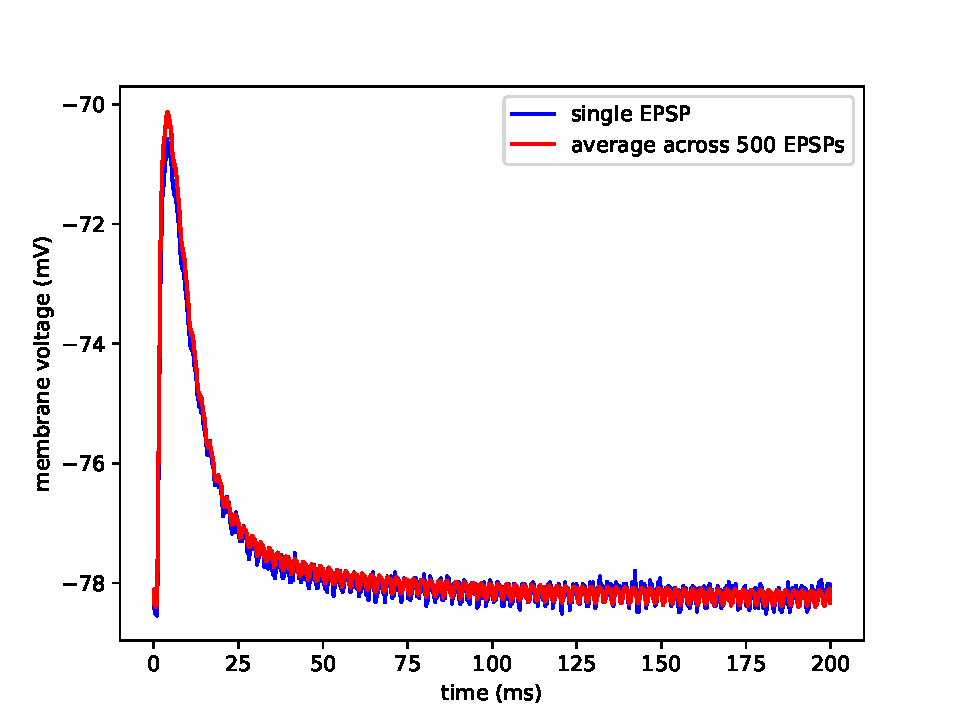
\includegraphics[width=.5\textwidth]{figures/epsp_out_+.pdf}
 %   \caption{EPSP for high drviout.}
 %   \label{fig:epsp_out+}
%\end{figure}
% \begin{figure}[ht]
%     \centering
%     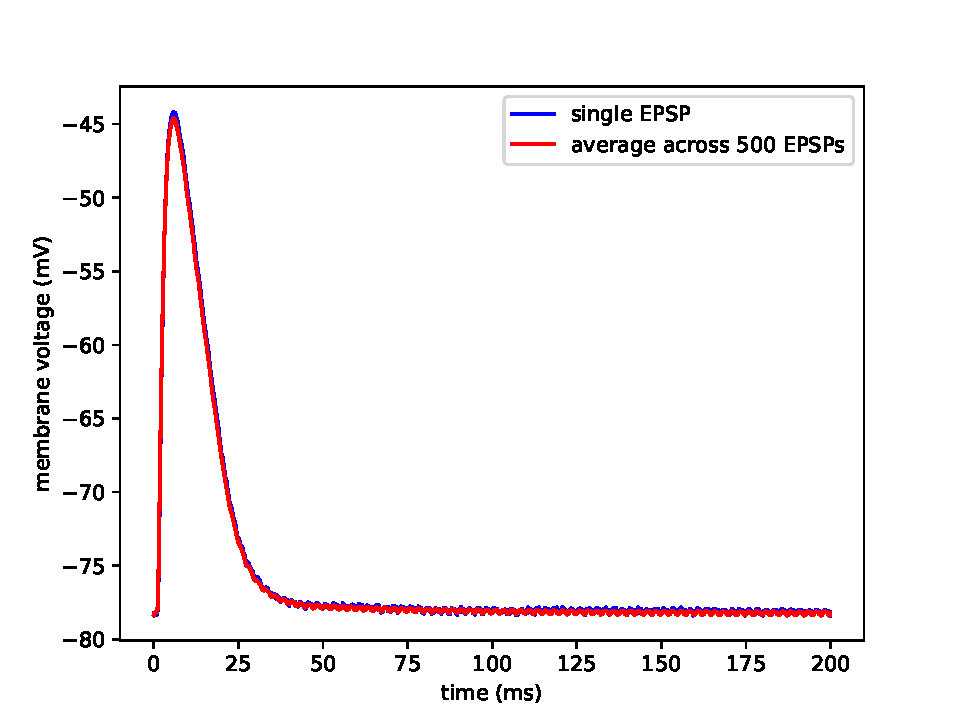
\includegraphics[width=.5\textwidth]{figures/epsp_fall_-.pdf}
%     \caption{EPSP for low drvifall.}
%     \label{fig:epsp_fall-}
% \end{figure}
%\begin{figure}[ht]
%    \centering
 %   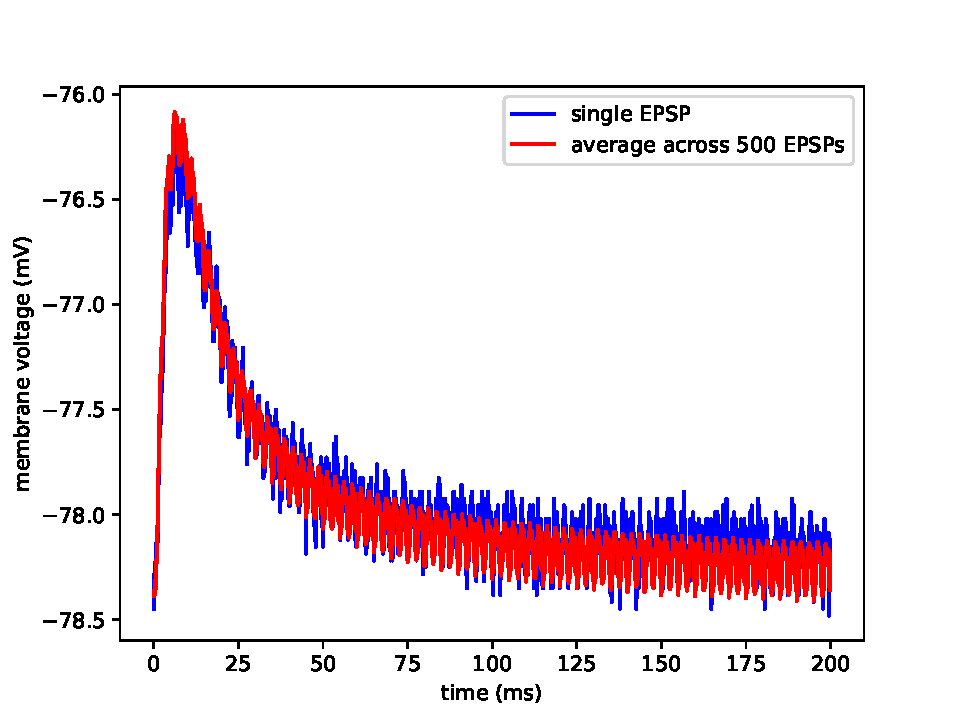
\includegraphics[width=.5\textwidth]{figures/epsp_fall_+.pdf}
 %   \caption{EPSP for high drvifall.}
 %   \label{fig:epsp_fall+}
%\end{figure}
We conclude that reducing drvifall leads to higher spikes while reducing drviout
leads to more slowly decaying (and lower) spikes.  \par
The ability of a neuron to perform computations (decisions) comes from the fact
that it can interpret specific spikes from input neurons as either suggesting
a likely decision (excitatory,  making spike more likely) or  a less likely decision
(inhibitory, making spike less likely).  We observe that changing the synapse type
leads to different post synaptic potentials.
\begin{figure}[ht]
    \centering
    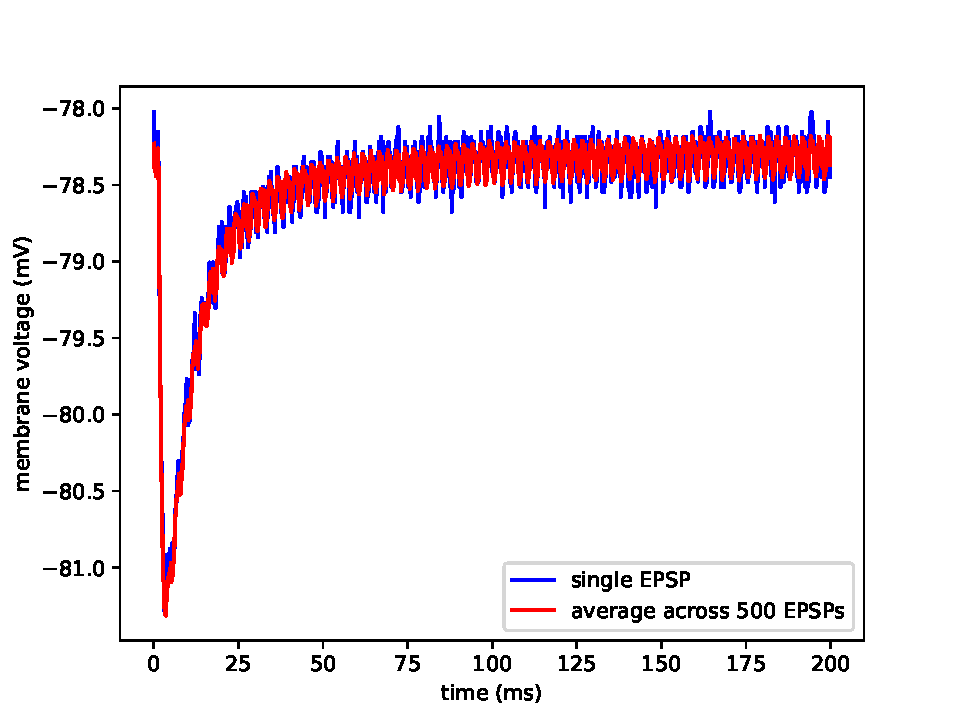
\includegraphics[width=.5\textwidth]{figures/epsp_inh_fall_03_out_05.pdf}
    \caption{EPSP for inhibitory neuron}
    \label{fig:epsp_inh_fall}
\end{figure}
\begin{figure}[ht]
    \centering
    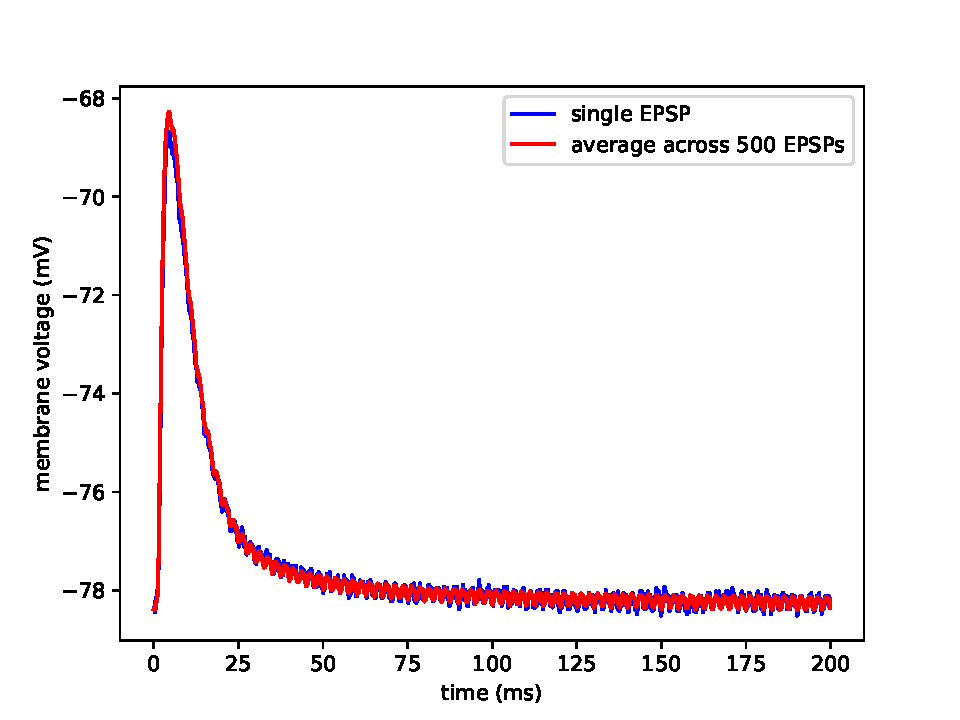
\includegraphics[width=.5\textwidth]{figures/epsp_exc_fall_03_out_05.pdf}
    \caption{EPSP for excitatory input}
    \label{fig:epsp_exc_fall}
\end{figure}
Note that for the same parameters,  the EPSP of the inhibitory neuron is much
smaller in magnitude than the one of the excitatory neuron.
It already became apparent that noise plays an important role (in fact it is very
strong for a single potential).  Two types of noise need to be distinguished here:
the temporal noise (different executions of the same process) and the neuron-to
neuron noise (fixed pattern; due to production errors).  A good measure of the neuron-
to-neuron noise is obtained by letting a neuron be stimulated by different synapses
and recording the resulting height of the voltage spike.  A median of $2.64$mV was
found with the considerable standard deviation of $1.17$mV.  This is shown in
\ref{MaxVoltHisto}.
\begin{figure}
		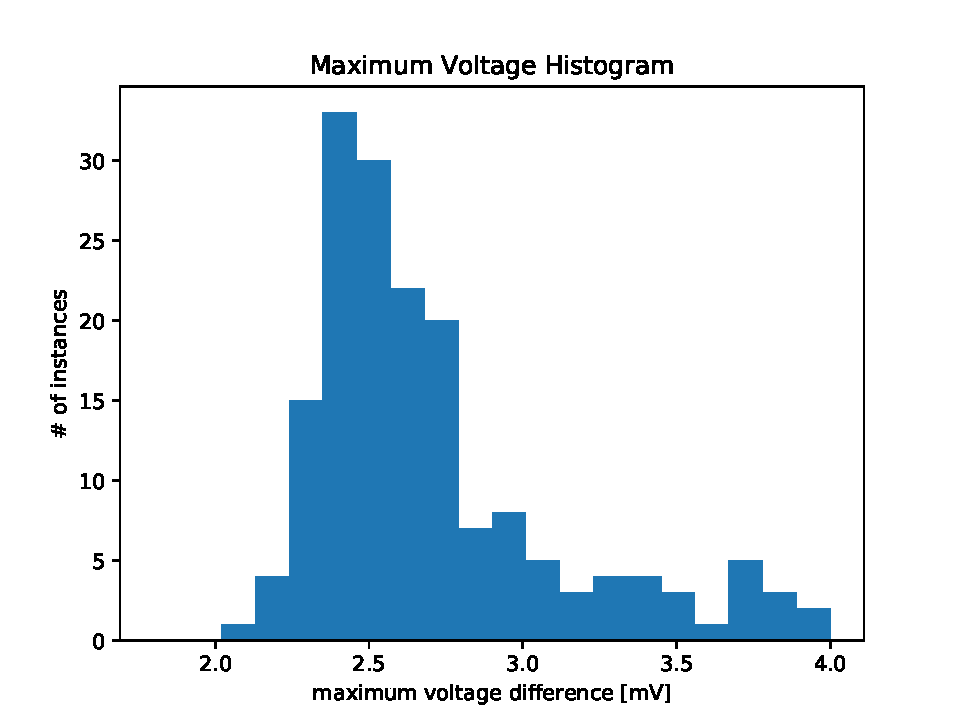
\includegraphics[width=0.5\textwidth]{figures/histo_maxVolt.pdf}
		\caption{Histogram of the peak heights for stimulation of different neurons}
		\label{MaxVoltHisto}
\end{figure}
To summarize,  it became apparent already for the simple case of single synaptic
input that while the chip behaves as expected and gives certain freedom in tuning
the response of neurons to input (thus allowing computations),  noise plays a very
significant role to such an extent that it will easily lead to wrong results when not
accounted for.
\subsection{Short Term Plasticity}
Short-term plasticity (STP) is a key feature of neurons that allows learning.
\textit{Plasticity} refers to the ability of changing synapse weights dynamically.
We implement short-term plasticity with a simplified Tsodyks-Markram model.  According
to this model,  neurotransmitters of a synapse are modeled as being in one of
three states: Recovered (\textbf{R}),  Effective (\textbf{E}),  Inactive
(\textbf{I}).  The behaviour of a synapse is determined by the parameters
$\tau_\text{rec}$ and $\tau_\text{facil}$ which govern the evolution according to
\begin{align*}
	R + E + I &= 1 \\
	\frac{dE}{dt} &= - \frac{E}{\tau_\text{facil}} + \sum_\text{spike} UR\delta(t-t_\text{spike} ) \\
	\frac{dR}{dt} &= + \frac{I}{\tau_\text{rec}} - \sum_\text{spike} UR\delta(t-t_\text{spike} ) \\
\end{align*}
As an example we show the membrane potential as a response to regularly
distributed spikes with a depressing mode in \ref{stp_depress}.  It can clearly be
seen how the neuron seems to ''remember'' its local history by reacting less sensitive
to spikes if they follow close to previous ones.  As expected from the theory,
the exponential decay of maximum voltage heights can be observed.  Again,  the response
can be controlled by choosing the activation $U$ and time constant $\tau$ accordingly.
\begin{figure}
		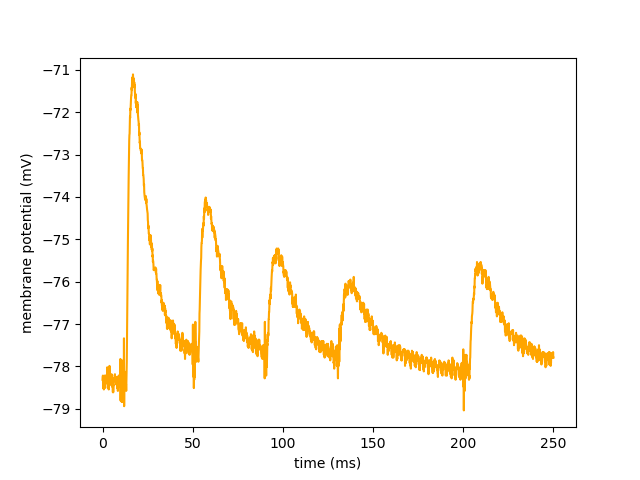
\includegraphics[width=.5\textwidth]{figures/stp_depressing.png}
		\label{stp_depress}
		\caption{Implementation of the depressing mode in short term plasticity}
\end{figure}

\subsection{Feed-Forward Networks}
\label{sec:feed-forward}
%% Robin  %%

%theory
One of the simplest neural networks one can consider is the feed-forward
network in which every neuron is arranged so that it passes on the signal it
receives to the next. In nature, a single neuron firing has relatively little
meaning until it is put in a larger context. Most of these contexts can be
simplified by viewing them as `superpositions' feed forward networks. It is
however important to consider that in nature robustness and redundancy is
highly favored in critical systems. The function of a feed-forward network can
be shutdown entirely if one neuron fails for whatever reason. Hence the concept
of populations is introduced, these are groups of neurons that perform the same
logical operations\footnote{That is to say, they are all either inhibitory or
excitatory neurons, they have the same neurons as inputs and the share the same
output neurons.} This is visualised in figure \ref{fig:feed-forward}.

\begin{figure}[ht]
    \centering
    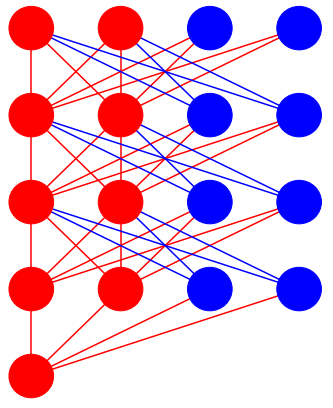
\includegraphics[width=.3\textwidth]{figures/feedforwardnetwork-cropped.png}
    \caption{Feed forward network with length 4 and population size 2. Two input
        neurons are drawn additionally. Exhibitory neurons and connections are drawn
        in red, inhibitory ones in blue.}
    \label{fig:feed-forward}
\end{figure}

In this experiment, connection weights also become relevant for the first time.
Any synaptic connection is assigned a weight, this weight represents the
membrane potential increase that a signal transfer induces. The importance of
this variable is crucial for networks as it nearly completely describes the
behaviour of a network.

%execution
A feed-forward network is described by the population number, the chain length
(see figure \ref{fig:feed-forward}) and the several weights of the following
type connections:
\begin{itemize}
    \item From the initial excitatory neuron to the first excitatory member of the
        chain. (ex0 $\rightarrow$ ex)
    \item From the initial excitatory neuron to the first inhibitory member of the
        chain. (ex0 $\rightarrow$ inh)
    \item From an excitatory neuron in the chain to the next excitatory neuron.
        (ex $\rightarrow$ ex)
    \item From an excitatory neuron in the chain to the next inhibitory neuron.
        (ex $\rightarrow$ inh)
    \item From an inhibitory neuron in the chain to the next excitatory neuron.
        (inh $\rightarrow$ ex)
\end{itemize}
This coincidentally is also the order of sensitivity (top being most sensitive),
particularly when discussing the `width' of the signal. With this is meant the
the amount of consequent signals that follow a single input signal. When having
a large population, a high (inh $\rightarrow$ ex) wheight was capable of
stopping the signal before it would reach the last neuron.

An issue that occurred as the chain length was increased the width of the signal
did as well. A length of 60 was reached creating a width of 10. This worked for
low populations, however with higher populations the membrane voltage was
overall raised to such a degree that the neurons started firing randomly and the
signal was lost. The theoretical maximum amount of neurons that could be used in
a chain is 192, so that for a population of size $n$ the max chain length
$c_\text{max}$ would be $c_\text{max} = 192 / n$.

An interesting phenomena occurs when the network is configured to loop. That is
to say the last neuron excites the first. Sadly it was not possible to set the
signal delay, which would have allowed for more careful investigation, but still
there was a clear effect visible in figure \ref{fig:feed-forward-loop}.

\begin{figure}
    \centering
    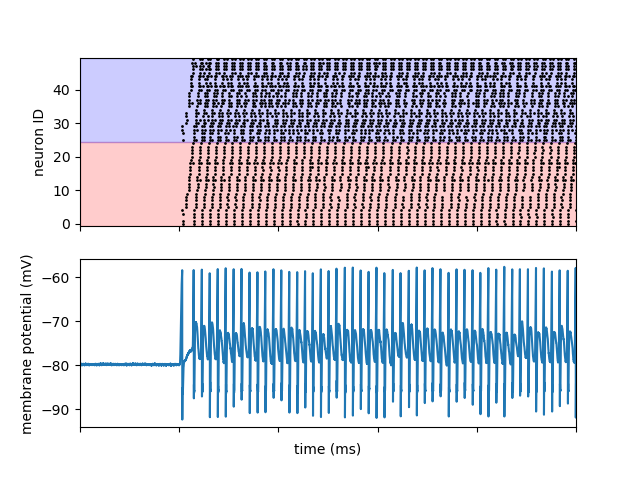
\includegraphics[width=.5\textwidth]{figures/feedforward signals loop.png}
    \caption{Feed-forward network configured in a loop. The population is 5, as
        is the chain length. Note that at the end the width starts to increase.
        The top figure shows all signals send by the neurons. The blue area
        represents inhibitory neurons, the red excitatory. The bottom figure
        shows the membrane potential of the first excitatory neuron.}
    \label{fig:feed-forward-loop}
\end{figure}

\subsection{Recurrent Networks}
We now construct a recurrent network with the connections sparse and random.
This adds some randomness to an otherwise regularly spiking neuron population.
Doing this produces a noise source that can be used for investigating other networks.
To determine the qualification of this setup as a noise source we check for certain
properties.  Typically,  the utilized noise is obtained from a Poisson process
that has a coefficient of variation
\begin{equation}
	CV = \frac{\sigma}{\mu} = 1
\end{equation}
with $\mu$ the mean and $\sigma$ the standard deviation. We first measure the
firing rate for each neuron and plot it against the CVs of inter-spike intervals.
\begin{figure}[ht]
    \centering
    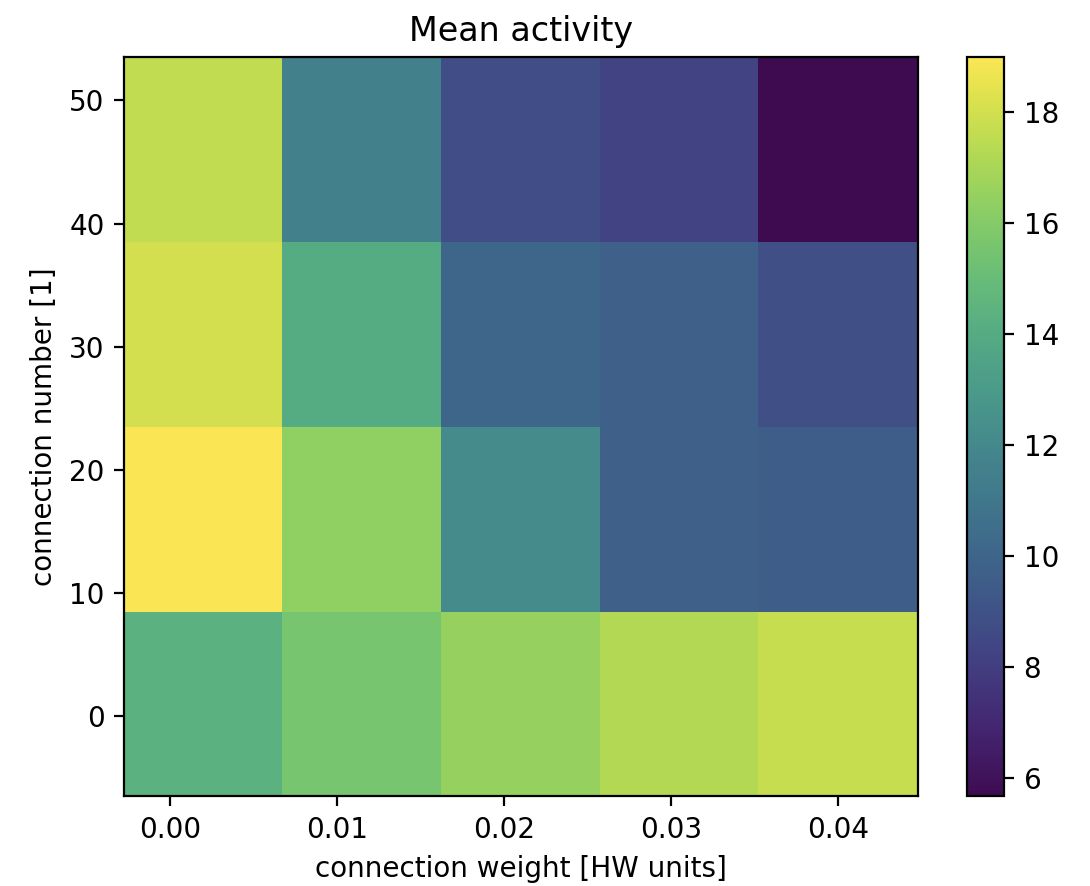
\includegraphics[width=.5\textwidth]{figures/activity_sweep.png}
    \caption{Parameter sweep of $w$ and $K$ to determine their effect on the activity 
    of the neurons.  Activity is encoded in the colour scheme shown on the z-axis.}
    \label{fig:activity_sweep}
\end{figure}
 %% insert 1.
Then we perform a parameter sweep on the weight $w$ and the number of presynaptic
partners $K$.  As expected, the mean activity decreases with connection weight
and connection number (since we have inhibitory synapses).  Similarly,  a parameter sweep
was done for the coefficient of variation.  Both procedures yield results with clear proportionalities
between the quantity of interest and connection weight and number.  The fact that it is possible
to find these relationships qualifies the SPIKEY chip as a noise source for other neuromorphic
devices since the average frequency of random spikes can be controlled (activity) and the type
of distribution can be chosen (defined by some CV).


\subsection{A Simple Computation: XOR}
A very common binary operation that is particularly non-linear (and therefore
more complex) is the XOR operation\cite{horowitz_hill_2020}.  A trivial solution
for this problem was found and dismissed thanks to its probable fragility.
Instead the institute provided a different network architecture that has
significant benefits over the suggested one: it is much more robust to what is
called referred to with `width' in section \ref{sec:feed-forward}. The
inhibitory neurons that are operating in a recurrent fashion prevent leaking
voltage from causing the any excitatory neuron in the network to fire out of
line. This is especially important in an XOR gate, as the chance that noise
would `cancel out' is negligible.

\begin{figure}
    \centering
    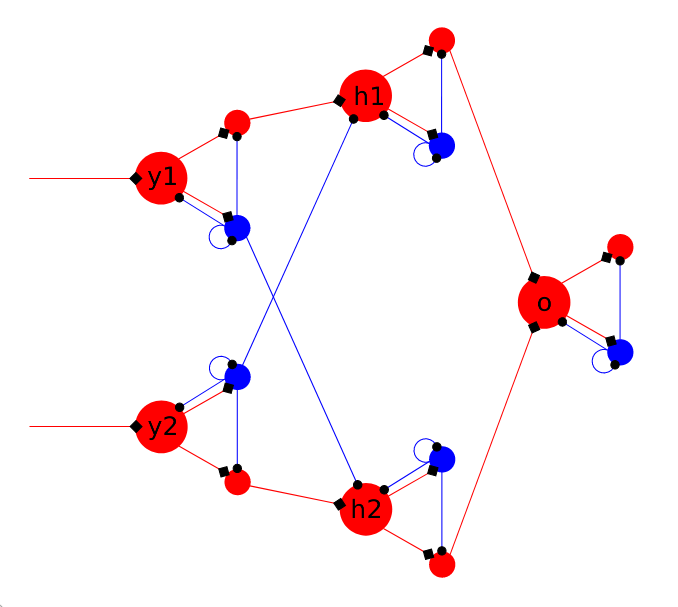
\includegraphics[width=.5\textwidth]{figures/XOR-used.png}
    \caption{Network that was used to test the ability of neurons to perform
        logical operations. Functions as an XOR gate.}
    \label{fig:XOR-used}
\end{figure}

A challenge that comes with a network like this is to find the correct set of
weights in order for the network to operate as expected. This was achieved by
plotting all signals sent in the same graph. This allowed for a speedy diagnosis
of the network by showing what expected signals were missing. An additional
script was present that would match the fired signals to expected time stamps,
giving a quantitative description of the quality of the network.

It quickly became clear that though a temporarily optimal configuration had been
found, it was not to last long, as a mere half hour later the accuracy had
dropped from 39/40 to 33/40. However the accuracy was large enough to show that
as the input was temporally shifted using a normal distribution, it did not
immediately lose it's accuracy. Only after the FWHM of the jitter became larger
than 15 milliseconds, the accuracy dropped below unrecognizable. This is
remarkable fact is likely due to the fact that the potential does not
immediately decay to the rest potential but remains high for some some time.
This could be useful in applications where signals are not perfectly timed, but
relative simultaneity is required.

\section{Conclusions}
Our results clearly show that the SPIKEY chip can be used for experimenting with
neuromorphic computing in the physical world. Most importantly, it could
verified that the elementary building block (LIF-circuit) behaved in a very
favourable way. Different characteristic features in different realizations of
that circuit in the hardware (due to production errors) can be observed but it
was shown to be possible to calibrate each  ``neuron'' in a way that the effect
of production errors is mostly cancelled. The circuit allows short term
plasticity,  a key trait of neurons that allows them to `learn'.  Finally,
leaving the few-neuron regime, it was verified that the hardware can be used to
model circuits with $\approx 200$ neurons, even binary logic was achievable with
the hardware.

However thanks to the temporal instability of the chip it is clearly not
production ready. It is hard to think of a critical application that would have
environmental conditions suited for this chip, that would be simultaneously cost
effective. Calibration would likely be sufficiently time consuming that it would
ruin any cost effectiveness. That is not to say that it is without application
in the world of research, where it can be a useful tool to investigate behaviour
of neural structures by making it behave like physical neurons.

\section{Discussion}
Comparing our quite complicated realization of the XOR-gate to the standard
electrical implementation of the binary gate in digital computing leads us to
one final important insight: When switching computer hardware to neuromorphic
hardware, it does not suffice to merely copy the brain's architecture and
continue to use boolean logic like it is done in conventional computers. It is
far too fragile, requiring an enormous amount of neurons and an inefficient use
of computation power.

Instead, if neuromorphic computing is to become an integral part of
computational methods, it is key the field adapts to the biological blueprint.
Naturally that would inspire radically new ways of problem solving in signal
processing.

Before that is reached however, a stark increase in the stability of the
hardware is required, as even a jelly fish has over 5000 neurons
\cite{neuronsjellyfish}. This paper has provided a qualitative review of the
chip, however quantitative measurements are still lacking. We hypothesize that
temporal differences in the internal temperature of the chip is likely the main
culprit of this instability, therefore describing both the sensitivity to a
change in temperature and heat generation by the chip during average usage could
be useful indicators of the chips ability to perform consistently.


\bibliography{main}
\bibliographystyle{plain}

\end{document}
